\section{Projektadministration}
Til at holde overblikket over opgaverne blev programmet Zenhub brugt. Dette er en add-on til Github, som er vores versionsstyringsværktøj. \\
Zenhub gør det muligt at have et elektronisk scrum board, hvor alle opgaver er oprettet, så begge gruppemedlemmer har et overblik over, har der mangler og hvad man arbejde med lige nu. \\
Et skærmbillde af scrum boardet i zenhub kan ses på figur \ref{fig:ZenhubScrum}.

\begin{figure} [H]
	\begin{center}
		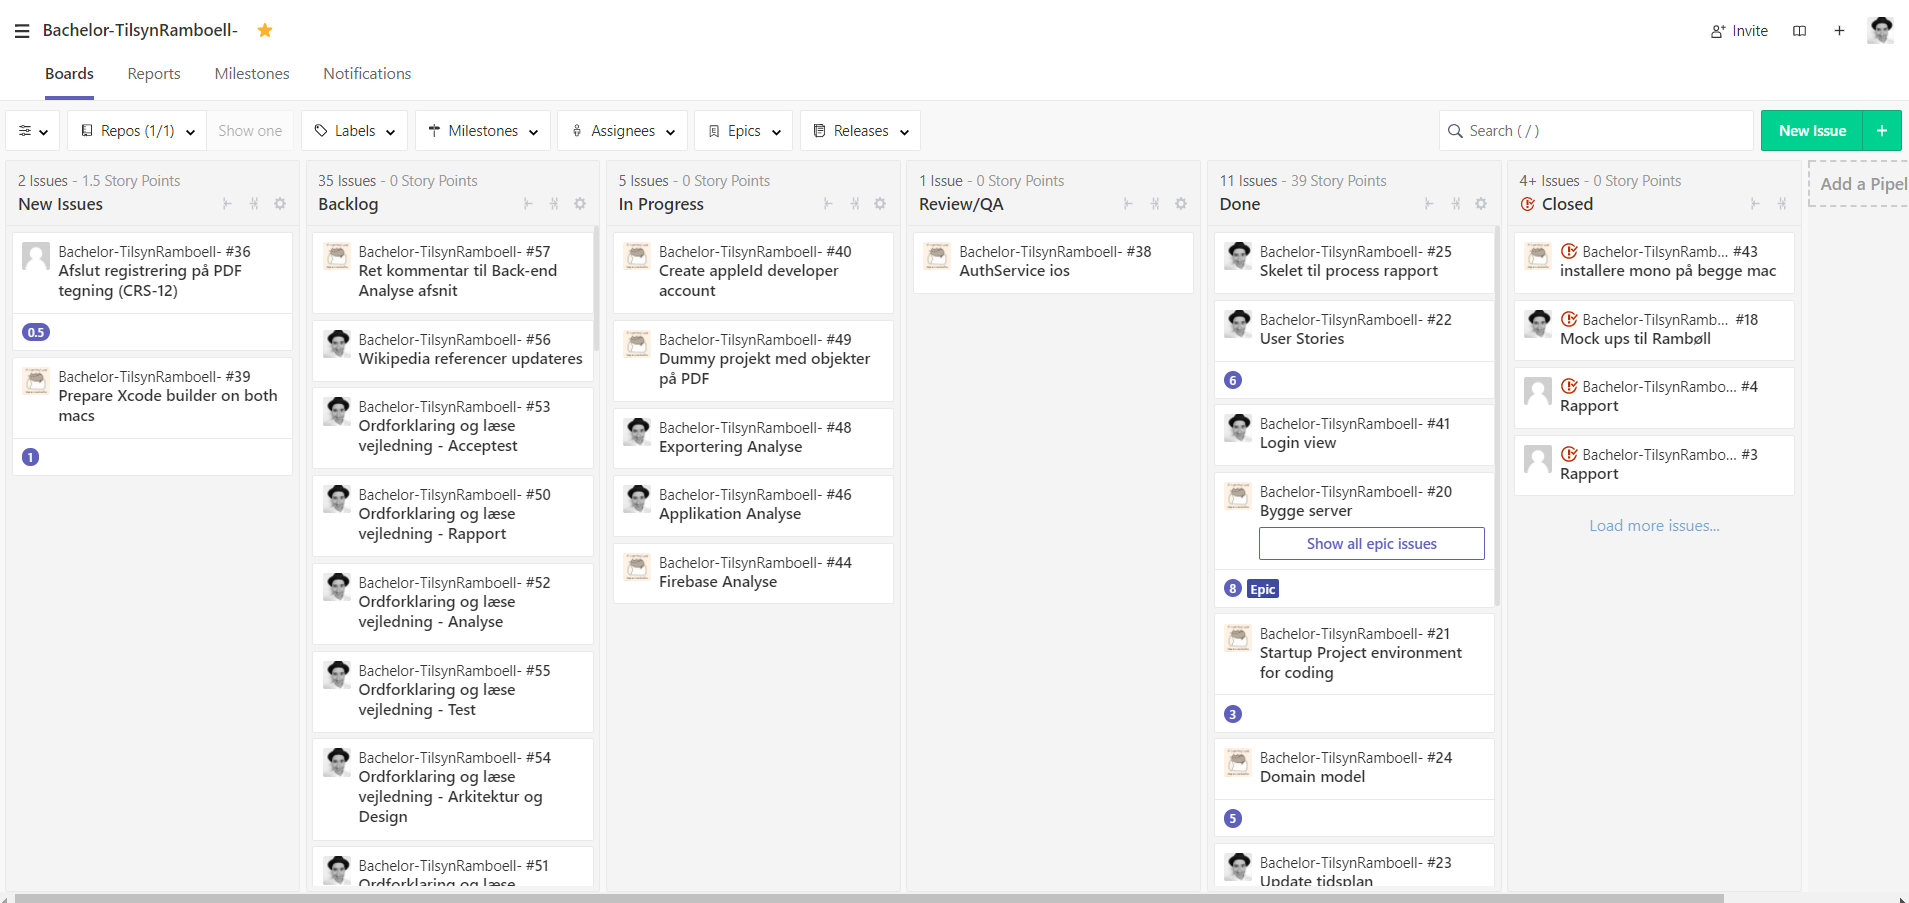
\includegraphics[height=8cm, width=15cm]{Projektadministration/Zenhub}
	\end{center}
	\caption{Scrum board i Zenhub.}
	\label{fig:ZenhubScrum}
\end{figure} 
